% Options for packages loaded elsewhere
\PassOptionsToPackage{unicode}{hyperref}
\PassOptionsToPackage{hyphens}{url}
%
\documentclass[
]{article}
\usepackage{lmodern}
\usepackage{amssymb,amsmath}
\usepackage{ifxetex,ifluatex}
\ifnum 0\ifxetex 1\fi\ifluatex 1\fi=0 % if pdftex
  \usepackage[T1]{fontenc}
  \usepackage[utf8]{inputenc}
  \usepackage{textcomp} % provide euro and other symbols
\else % if luatex or xetex
  \usepackage{unicode-math}
  \defaultfontfeatures{Scale=MatchLowercase}
  \defaultfontfeatures[\rmfamily]{Ligatures=TeX,Scale=1}
\fi
% Use upquote if available, for straight quotes in verbatim environments
\IfFileExists{upquote.sty}{\usepackage{upquote}}{}
\IfFileExists{microtype.sty}{% use microtype if available
  \usepackage[]{microtype}
  \UseMicrotypeSet[protrusion]{basicmath} % disable protrusion for tt fonts
}{}
\makeatletter
\@ifundefined{KOMAClassName}{% if non-KOMA class
  \IfFileExists{parskip.sty}{%
    \usepackage{parskip}
  }{% else
    \setlength{\parindent}{0pt}
    \setlength{\parskip}{6pt plus 2pt minus 1pt}}
}{% if KOMA class
  \KOMAoptions{parskip=half}}
\makeatother
\usepackage{xcolor}
\IfFileExists{xurl.sty}{\usepackage{xurl}}{} % add URL line breaks if available
\IfFileExists{bookmark.sty}{\usepackage{bookmark}}{\usepackage{hyperref}}
\hypersetup{
  pdftitle={HW1 - STA 135},
  pdfauthor={Gianni Spiga},
  hidelinks,
  pdfcreator={LaTeX via pandoc}}
\urlstyle{same} % disable monospaced font for URLs
\usepackage[margin=1in]{geometry}
\usepackage{color}
\usepackage{fancyvrb}
\newcommand{\VerbBar}{|}
\newcommand{\VERB}{\Verb[commandchars=\\\{\}]}
\DefineVerbatimEnvironment{Highlighting}{Verbatim}{commandchars=\\\{\}}
% Add ',fontsize=\small' for more characters per line
\usepackage{framed}
\definecolor{shadecolor}{RGB}{248,248,248}
\newenvironment{Shaded}{\begin{snugshade}}{\end{snugshade}}
\newcommand{\AlertTok}[1]{\textcolor[rgb]{0.94,0.16,0.16}{#1}}
\newcommand{\AnnotationTok}[1]{\textcolor[rgb]{0.56,0.35,0.01}{\textbf{\textit{#1}}}}
\newcommand{\AttributeTok}[1]{\textcolor[rgb]{0.77,0.63,0.00}{#1}}
\newcommand{\BaseNTok}[1]{\textcolor[rgb]{0.00,0.00,0.81}{#1}}
\newcommand{\BuiltInTok}[1]{#1}
\newcommand{\CharTok}[1]{\textcolor[rgb]{0.31,0.60,0.02}{#1}}
\newcommand{\CommentTok}[1]{\textcolor[rgb]{0.56,0.35,0.01}{\textit{#1}}}
\newcommand{\CommentVarTok}[1]{\textcolor[rgb]{0.56,0.35,0.01}{\textbf{\textit{#1}}}}
\newcommand{\ConstantTok}[1]{\textcolor[rgb]{0.00,0.00,0.00}{#1}}
\newcommand{\ControlFlowTok}[1]{\textcolor[rgb]{0.13,0.29,0.53}{\textbf{#1}}}
\newcommand{\DataTypeTok}[1]{\textcolor[rgb]{0.13,0.29,0.53}{#1}}
\newcommand{\DecValTok}[1]{\textcolor[rgb]{0.00,0.00,0.81}{#1}}
\newcommand{\DocumentationTok}[1]{\textcolor[rgb]{0.56,0.35,0.01}{\textbf{\textit{#1}}}}
\newcommand{\ErrorTok}[1]{\textcolor[rgb]{0.64,0.00,0.00}{\textbf{#1}}}
\newcommand{\ExtensionTok}[1]{#1}
\newcommand{\FloatTok}[1]{\textcolor[rgb]{0.00,0.00,0.81}{#1}}
\newcommand{\FunctionTok}[1]{\textcolor[rgb]{0.00,0.00,0.00}{#1}}
\newcommand{\ImportTok}[1]{#1}
\newcommand{\InformationTok}[1]{\textcolor[rgb]{0.56,0.35,0.01}{\textbf{\textit{#1}}}}
\newcommand{\KeywordTok}[1]{\textcolor[rgb]{0.13,0.29,0.53}{\textbf{#1}}}
\newcommand{\NormalTok}[1]{#1}
\newcommand{\OperatorTok}[1]{\textcolor[rgb]{0.81,0.36,0.00}{\textbf{#1}}}
\newcommand{\OtherTok}[1]{\textcolor[rgb]{0.56,0.35,0.01}{#1}}
\newcommand{\PreprocessorTok}[1]{\textcolor[rgb]{0.56,0.35,0.01}{\textit{#1}}}
\newcommand{\RegionMarkerTok}[1]{#1}
\newcommand{\SpecialCharTok}[1]{\textcolor[rgb]{0.00,0.00,0.00}{#1}}
\newcommand{\SpecialStringTok}[1]{\textcolor[rgb]{0.31,0.60,0.02}{#1}}
\newcommand{\StringTok}[1]{\textcolor[rgb]{0.31,0.60,0.02}{#1}}
\newcommand{\VariableTok}[1]{\textcolor[rgb]{0.00,0.00,0.00}{#1}}
\newcommand{\VerbatimStringTok}[1]{\textcolor[rgb]{0.31,0.60,0.02}{#1}}
\newcommand{\WarningTok}[1]{\textcolor[rgb]{0.56,0.35,0.01}{\textbf{\textit{#1}}}}
\usepackage{graphicx,grffile}
\makeatletter
\def\maxwidth{\ifdim\Gin@nat@width>\linewidth\linewidth\else\Gin@nat@width\fi}
\def\maxheight{\ifdim\Gin@nat@height>\textheight\textheight\else\Gin@nat@height\fi}
\makeatother
% Scale images if necessary, so that they will not overflow the page
% margins by default, and it is still possible to overwrite the defaults
% using explicit options in \includegraphics[width, height, ...]{}
\setkeys{Gin}{width=\maxwidth,height=\maxheight,keepaspectratio}
% Set default figure placement to htbp
\makeatletter
\def\fps@figure{htbp}
\makeatother
\setlength{\emergencystretch}{3em} % prevent overfull lines
\providecommand{\tightlist}{%
  \setlength{\itemsep}{0pt}\setlength{\parskip}{0pt}}
\setcounter{secnumdepth}{-\maxdimen} % remove section numbering

\title{HW1 - STA 135}
\author{Gianni Spiga}
\date{3/29/2022}

\begin{document}
\maketitle

\hypertarget{problem-1.6}{%
\subsection{Problem 1.6}\label{problem-1.6}}

\hypertarget{a.}{%
\subsubsection{a.)}\label{a.}}

\begin{Shaded}
\begin{Highlighting}[]
\NormalTok{airpol <-}
\StringTok{  }\KeywordTok{read.csv}\NormalTok{(}\StringTok{"~/GitHub/STA135/Homework/HW1/Air-Pollution Data G.C.Tao.csv"}\NormalTok{,}
           \DataTypeTok{header =} \OtherTok{TRUE}\NormalTok{)}
\KeywordTok{library}\NormalTok{(ggplot2)}
\KeywordTok{library}\NormalTok{(ggExtra)}
\KeywordTok{library}\NormalTok{(GGally)}
\end{Highlighting}
\end{Shaded}

\begin{verbatim}
## Registered S3 method overwritten by 'GGally':
##   method from   
##   +.gg   ggplot2
\end{verbatim}

\begin{Shaded}
\begin{Highlighting}[]
\CommentTok{#Pairwise plots}
\KeywordTok{ggpairs}\NormalTok{(airpol)}
\end{Highlighting}
\end{Shaded}

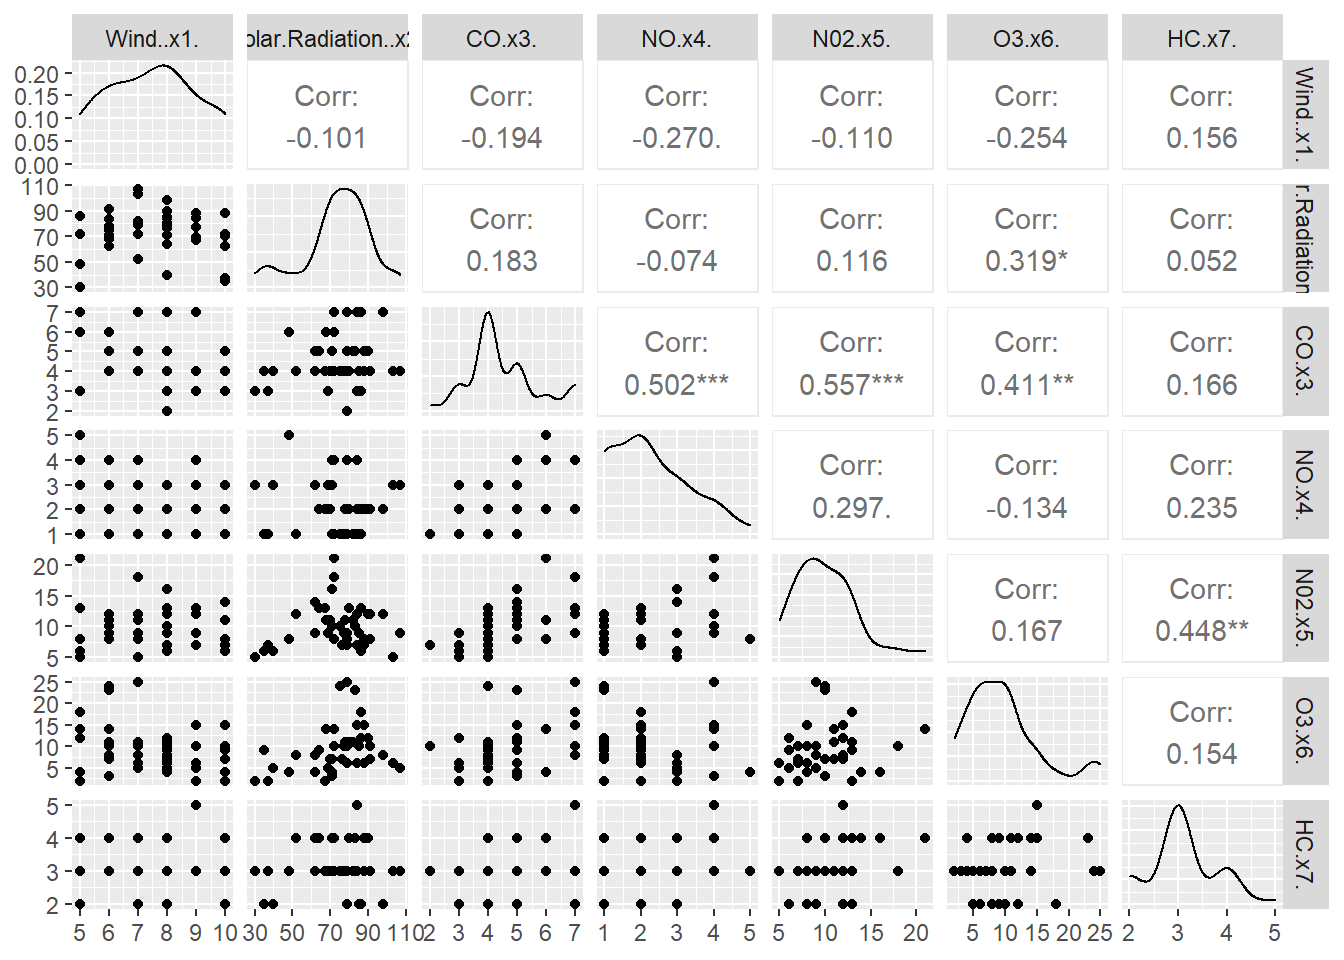
\includegraphics{HW1_files/figure-latex/unnamed-chunk-1-1.pdf}

\begin{Shaded}
\begin{Highlighting}[]
\CommentTok{#Marginal plots}
\CommentTok{# colnames <- names(airpol)}
\CommentTok{# for (i in colnames[-1])\{}
\CommentTok{#   print(ggMarginal(ggplot(airpol, aes_string(x = "Wind..x1.", y = i)) + geom_point(color = 'firebrick'), type = 'histogram', fill = 'dodgerblue'))}
\CommentTok{# \}}
\end{Highlighting}
\end{Shaded}

\hypertarget{b.}{%
\subsubsection{b.)}\label{b.}}

\begin{Shaded}
\begin{Highlighting}[]
\CommentTok{#xbar, mean vector}
\KeywordTok{colMeans}\NormalTok{(airpol[}\KeywordTok{sapply}\NormalTok{(airpol, is.numeric)]) }
\end{Highlighting}
\end{Shaded}

\begin{verbatim}
##            Wind..x1. Solar.Radiation..x2.               CO.x3. 
##             7.500000            73.857143             4.547619 
##               NO.x4.              N02.x5.               O3.x6. 
##             2.190476            10.047619             9.404762 
##               HC.x7. 
##             3.095238
\end{verbatim}

\begin{Shaded}
\begin{Highlighting}[]
\CommentTok{#Sn, the COV/VAR marix}
\NormalTok{n =}\StringTok{ }\KeywordTok{nrow}\NormalTok{(airpol)}
\KeywordTok{cov}\NormalTok{(airpol) }\OperatorTok{*}\StringTok{ }\NormalTok{(n}\DecValTok{-1}\NormalTok{)}\OperatorTok{/}\NormalTok{n}
\end{Highlighting}
\end{Shaded}

\begin{verbatim}
##                       Wind..x1. Solar.Radiation..x2.     CO.x3.     NO.x4.
## Wind..x1.             2.4404762           -2.7142857 -0.3690476 -0.4523810
## Solar.Radiation..x2. -2.7142857          293.3605442  3.8163265 -1.3537415
## CO.x3.               -0.3690476            3.8163265  1.4858277  0.6575964
## NO.x4.               -0.4523810           -1.3537415  0.6575964  1.1541950
## N02.x5.              -0.5714286            6.6020408  2.2596372  1.0623583
## O3.x6.               -2.1785714           30.0578231  2.7545351 -0.7913832
## HC.x7.                0.1666667            0.6088435  0.1383220  0.1723356
##                         N02.x5.     O3.x6.    HC.x7.
## Wind..x1.            -0.5714286 -2.1785714 0.1666667
## Solar.Radiation..x2.  6.6020408 30.0578231 0.6088435
## CO.x3.                2.2596372  2.7545351 0.1383220
## NO.x4.                1.0623583 -0.7913832 0.1723356
## N02.x5.              11.0929705  3.0521542 1.0192744
## O3.x6.                3.0521542 30.2409297 0.5804989
## HC.x7.                1.0192744  0.5804989 0.4671202
\end{verbatim}

\begin{Shaded}
\begin{Highlighting}[]
\CommentTok{# R the correlation matrix}
\KeywordTok{round}\NormalTok{(}\KeywordTok{cor}\NormalTok{(airpol),}\DecValTok{2}\NormalTok{)}
\end{Highlighting}
\end{Shaded}

\begin{verbatim}
##                      Wind..x1. Solar.Radiation..x2. CO.x3. NO.x4. N02.x5.
## Wind..x1.                 1.00                -0.10  -0.19  -0.27   -0.11
## Solar.Radiation..x2.     -0.10                 1.00   0.18  -0.07    0.12
## CO.x3.                   -0.19                 0.18   1.00   0.50    0.56
## NO.x4.                   -0.27                -0.07   0.50   1.00    0.30
## N02.x5.                  -0.11                 0.12   0.56   0.30    1.00
## O3.x6.                   -0.25                 0.32   0.41  -0.13    0.17
## HC.x7.                    0.16                 0.05   0.17   0.23    0.45
##                      O3.x6. HC.x7.
## Wind..x1.             -0.25   0.16
## Solar.Radiation..x2.   0.32   0.05
## CO.x3.                 0.41   0.17
## NO.x4.                -0.13   0.23
## N02.x5.                0.17   0.45
## O3.x6.                 1.00   0.15
## HC.x7.                 0.15   1.00
\end{verbatim}

We can see that none of the variables have a very high correlation. We
can see the highest correlation in our data is between Carbon Monoxide
(CO) and Nitrogen Dioxide (NO2) of 0.557. We also can see that Wind is
negatively correlated with all pollutants.

\hypertarget{problem-1.9}{%
\subsection{Problem 1.9}\label{problem-1.9}}

\begin{Shaded}
\begin{Highlighting}[]
\CommentTok{#a.)}
\KeywordTok{library}\NormalTok{(plotly)}
\end{Highlighting}
\end{Shaded}

\begin{verbatim}
## 
## Attaching package: 'plotly'
\end{verbatim}

\begin{verbatim}
## The following object is masked from 'package:ggplot2':
## 
##     last_plot
\end{verbatim}

\begin{verbatim}
## The following object is masked from 'package:stats':
## 
##     filter
\end{verbatim}

\begin{verbatim}
## The following object is masked from 'package:graphics':
## 
##     layout
\end{verbatim}

\begin{Shaded}
\begin{Highlighting}[]
\NormalTok{x1 <-}\StringTok{ }\KeywordTok{c}\NormalTok{(}\OperatorTok{-}\DecValTok{6}\NormalTok{, }\DecValTok{-3}\NormalTok{, }\DecValTok{-2}\NormalTok{, }\DecValTok{1}\NormalTok{, }\DecValTok{2}\NormalTok{, }\DecValTok{5}\NormalTok{, }\DecValTok{6}\NormalTok{, }\DecValTok{8}\NormalTok{)}
\NormalTok{x2 <-}\StringTok{ }\KeywordTok{c}\NormalTok{(}\OperatorTok{-}\DecValTok{2}\NormalTok{, }\DecValTok{-3}\NormalTok{, }\DecValTok{1}\NormalTok{, }\DecValTok{-1}\NormalTok{, }\DecValTok{2}\NormalTok{, }\DecValTok{1}\NormalTok{, }\DecValTok{5}\NormalTok{, }\DecValTok{3}\NormalTok{)}
\NormalTok{mydata <-}\StringTok{ }\KeywordTok{data.frame}\NormalTok{(x1, x2)}

\CommentTok{#ggplot(aes(x = x1, y = x2)) + geom_point()}
\NormalTok{fig <-}\StringTok{ }\KeywordTok{plot_ly}\NormalTok{(mydata, }\DataTypeTok{x =} \OperatorTok{~}\NormalTok{x1, }\DataTypeTok{y =} \OperatorTok{~}\NormalTok{x2)}
\NormalTok{fig}
\end{Highlighting}
\end{Shaded}

\begin{verbatim}
## No trace type specified:
##   Based on info supplied, a 'scatter' trace seems appropriate.
##   Read more about this trace type -> https://plotly.com/r/reference/#scatter
\end{verbatim}

\begin{verbatim}
## No scatter mode specifed:
##   Setting the mode to markers
##   Read more about this attribute -> https://plotly.com/r/reference/#scatter-mode
\end{verbatim}

\begin{Shaded}
\begin{Highlighting}[]
\NormalTok{n =}\StringTok{ }\KeywordTok{nrow}\NormalTok{(mydata)}
\NormalTok{myvarmat =}\StringTok{ }\KeywordTok{cov}\NormalTok{(mydata) }\OperatorTok{*}\StringTok{ }\NormalTok{(n}\DecValTok{-1}\NormalTok{)}\OperatorTok{/}\NormalTok{n}
\NormalTok{myvarmat}
\end{Highlighting}
\end{Shaded}

\begin{verbatim}
##          x1      x2
## x1 20.48438 9.09375
## x2  9.09375 6.18750
\end{verbatim}

\begin{Shaded}
\begin{Highlighting}[]
\NormalTok{s11 =}\StringTok{ }\NormalTok{myvarmat[}\DecValTok{1}\NormalTok{]}
\NormalTok{s12 =}\StringTok{ }\NormalTok{myvarmat[}\DecValTok{2}\NormalTok{]}
\NormalTok{s22 =}\StringTok{ }\NormalTok{myvarmat[}\DecValTok{4}\NormalTok{]}
\end{Highlighting}
\end{Shaded}

\begin{Shaded}
\begin{Highlighting}[]
\CommentTok{#b.) }
\CommentTok{#Formula pdf page 56}

\CommentTok{# x1~ = x1 costheta + x2 sintheta}
\NormalTok{x1tilde =}\StringTok{ }\NormalTok{x1 }\OperatorTok{*}\StringTok{ }\FloatTok{0.899} \OperatorTok{+}\StringTok{ }\NormalTok{x2 }\OperatorTok{*}\StringTok{ }\FloatTok{0.438}

\CommentTok{# x2~ = -x1 sintheta + x2 costheta}
\NormalTok{x2tilde =}\StringTok{ }\OperatorTok{-}\NormalTok{x1 }\OperatorTok{*}\StringTok{ }\FloatTok{0.438} \OperatorTok{+}\StringTok{ }\NormalTok{x2 }\OperatorTok{*}\StringTok{ }\FloatTok{0.899}

\CommentTok{#c }
\NormalTok{datatilde =}\StringTok{ }\KeywordTok{data.frame}\NormalTok{(x1tilde, x2tilde)}
\NormalTok{n =}\StringTok{ }\KeywordTok{nrow}\NormalTok{(datatilde)}
\KeywordTok{diag}\NormalTok{(}\KeywordTok{var}\NormalTok{(datatilde))  }\CommentTok{#* (n-1)/n)}
\end{Highlighting}
\end{Shaded}

\begin{verbatim}
##   x1tilde   x2tilde 
## 28.461798  2.021716
\end{verbatim}

\begin{Shaded}
\begin{Highlighting}[]
\CommentTok{#d}
\NormalTok{newx1 =}\StringTok{ }\DecValTok{4} \OperatorTok{*}\StringTok{ }\FloatTok{0.899} \OperatorTok{+}\StringTok{ }\DecValTok{-2} \OperatorTok{*}\StringTok{ }\FloatTok{0.438}
\NormalTok{newx2 =}\StringTok{ }\DecValTok{-4} \OperatorTok{*}\StringTok{ }\FloatTok{0.438} \OperatorTok{+}\StringTok{ }\DecValTok{-2} \OperatorTok{*}\StringTok{ }\FloatTok{0.899}

\NormalTok{dOP =}\StringTok{ }\KeywordTok{sqrt}\NormalTok{((newx1}\OperatorTok{^}\DecValTok{2}\OperatorTok{/}\FloatTok{28.462}\NormalTok{) }\OperatorTok{+}\StringTok{ }\NormalTok{(newx2}\OperatorTok{^}\DecValTok{2}\OperatorTok{/}\FloatTok{2.022}\NormalTok{))}
\NormalTok{dOP}
\end{Highlighting}
\end{Shaded}

\begin{verbatim}
## [1] 2.548064
\end{verbatim}

\begin{Shaded}
\begin{Highlighting}[]
\CommentTok{#e}
\CommentTok{#From footnote}
\NormalTok{a11 =}\StringTok{ }\NormalTok{(}\FloatTok{0.899}\OperatorTok{^}\DecValTok{2}\OperatorTok{/}\NormalTok{(}\FloatTok{0.899}\OperatorTok{^}\DecValTok{2} \OperatorTok{*}\StringTok{ }\NormalTok{s11 }\OperatorTok{+}\StringTok{ }\DecValTok{2} \OperatorTok{*}\StringTok{ }\FloatTok{0.438} \OperatorTok{*}\StringTok{ }\FloatTok{0.899} \OperatorTok{*}\StringTok{ }\NormalTok{s12 }\OperatorTok{+}\StringTok{ }\FloatTok{0.438}\OperatorTok{^}\DecValTok{2} \OperatorTok{*}\StringTok{ }\NormalTok{s22)) }\OperatorTok{+}\StringTok{ }\NormalTok{(}\FloatTok{0.438}\OperatorTok{^}\DecValTok{2}\OperatorTok{/}\StringTok{ }\NormalTok{(}\FloatTok{0.899}\OperatorTok{^}\DecValTok{2} \OperatorTok{*}\StringTok{ }\NormalTok{s22 }\OperatorTok{-}\StringTok{ }\DecValTok{2} \OperatorTok{*}\StringTok{ }\FloatTok{0.438} \OperatorTok{*}\StringTok{ }\FloatTok{0.899} \OperatorTok{*}\StringTok{ }\NormalTok{s12 }\OperatorTok{+}\StringTok{ }\FloatTok{0.438}\OperatorTok{^}\DecValTok{2} \OperatorTok{*}\StringTok{ }\NormalTok{s11))}

\NormalTok{a22 =}\StringTok{ }\NormalTok{(}\FloatTok{0.438}\OperatorTok{^}\DecValTok{2} \OperatorTok{/}\StringTok{ }\NormalTok{(}\FloatTok{0.899}\OperatorTok{^}\DecValTok{2} \OperatorTok{*}\StringTok{ }\NormalTok{s11 }\OperatorTok{+}\StringTok{ }\DecValTok{2} \OperatorTok{*}\StringTok{ }\FloatTok{0.438} \OperatorTok{*}\StringTok{ }\FloatTok{0.899} \OperatorTok{*}\NormalTok{s12 }\OperatorTok{+}\StringTok{ }\FloatTok{0.438}\OperatorTok{^}\DecValTok{2} \OperatorTok{*}\StringTok{ }\NormalTok{s22)) }\OperatorTok{+}\StringTok{ }\NormalTok{(}\FloatTok{0.899}\OperatorTok{^}\DecValTok{2} \OperatorTok{/}\StringTok{ }\NormalTok{(}\FloatTok{0.899}\OperatorTok{^}\DecValTok{2} \OperatorTok{*}\StringTok{ }\NormalTok{s22 }\OperatorTok{-}\StringTok{ }\DecValTok{2} \OperatorTok{*}\StringTok{ }\FloatTok{0.438} \OperatorTok{*}\StringTok{ }\FloatTok{0.899}\OperatorTok{*}\NormalTok{s12 }\OperatorTok{+}\StringTok{ }\FloatTok{0.438}\OperatorTok{^}\DecValTok{2} \OperatorTok{*}\StringTok{ }\NormalTok{s11))}

\NormalTok{a12 =}\StringTok{ }\NormalTok{((}\FloatTok{0.438} \OperatorTok{*}\StringTok{ }\FloatTok{0.899}\NormalTok{) }\OperatorTok{/}\StringTok{ }\NormalTok{(}\FloatTok{0.899}\OperatorTok{^}\DecValTok{2} \OperatorTok{*}\StringTok{ }\NormalTok{s11 }\OperatorTok{+}\StringTok{ }\DecValTok{2} \OperatorTok{*}\StringTok{ }\FloatTok{0.438} \OperatorTok{*}\StringTok{ }\FloatTok{0.899} \OperatorTok{*}\StringTok{ }\NormalTok{s12 }\OperatorTok{+}\StringTok{ }\FloatTok{0.438}\OperatorTok{^}\DecValTok{2} \OperatorTok{*}\StringTok{ }\NormalTok{s22)) }\OperatorTok{-}\StringTok{ }\NormalTok{((}\FloatTok{0.438} \OperatorTok{*}\StringTok{ }\FloatTok{0.899}\NormalTok{)}\OperatorTok{/}\StringTok{ }\NormalTok{(}\FloatTok{0.899}\OperatorTok{^}\DecValTok{2} \OperatorTok{*}\StringTok{ }\NormalTok{s22 }\OperatorTok{-}\StringTok{ }\DecValTok{2} \OperatorTok{*}\StringTok{ }\FloatTok{0.438} \OperatorTok{*}\StringTok{ }\FloatTok{0.899} \OperatorTok{*}\StringTok{ }\NormalTok{s12 }\OperatorTok{+}\StringTok{ }\FloatTok{0.438}\OperatorTok{^}\DecValTok{2} \OperatorTok{*}\StringTok{ }\NormalTok{s11))}

\NormalTok{dOP2 =}\StringTok{ }\KeywordTok{sqrt}\NormalTok{((a11 }\OperatorTok{*}\StringTok{ }\DecValTok{16}\NormalTok{) }\OperatorTok{+}\StringTok{ }\NormalTok{(}\DecValTok{2}\OperatorTok{*}\NormalTok{a12 }\OperatorTok{*}\StringTok{ }\DecValTok{4} \OperatorTok{*}\StringTok{ }\DecValTok{-2}\NormalTok{) }\OperatorTok{+}\StringTok{ }\NormalTok{(a22 }\OperatorTok{*}\StringTok{ }\DecValTok{4}\NormalTok{))}
\NormalTok{dOP2}
\end{Highlighting}
\end{Shaded}

\begin{verbatim}
## [1] 2.724179
\end{verbatim}

We can see that within rounding error, these two distances are about the
same.

\hypertarget{p-1.18}{%
\subsection{P 1.18}\label{p-1.18}}

\begin{Shaded}
\begin{Highlighting}[]
\NormalTok{WomenTrack <-}\StringTok{ }\KeywordTok{read.csv}\NormalTok{(}\StringTok{"~/Github/STA135/Homework/HW1/National Track Records for Women.csv"}\NormalTok{, }\DataTypeTok{header =}  \OtherTok{TRUE}\NormalTok{)}
\CommentTok{#WomenTrack}

\CommentTok{#First, convert last 4 columns into seconds }
\NormalTok{WomenTrack[,}\DecValTok{5}\OperatorTok{:}\DecValTok{8}\NormalTok{] =}\StringTok{ }\NormalTok{WomenTrack[, }\DecValTok{5}\OperatorTok{:}\DecValTok{8}\NormalTok{] }\OperatorTok{*}\StringTok{ }\DecValTok{60}
\CommentTok{#WomenTrack}

\CommentTok{#Second, divide each column by respective meters to get meters per second}
\NormalTok{meters =}\StringTok{ }\KeywordTok{c}\NormalTok{(}\DecValTok{1}\NormalTok{, }\DecValTok{100}\NormalTok{, }\DecValTok{200}\NormalTok{, }\DecValTok{400}\NormalTok{, }\DecValTok{800}\NormalTok{, }\DecValTok{1500}\NormalTok{, }\DecValTok{3000}\NormalTok{, }\DecValTok{42195}\NormalTok{)}
\ControlFlowTok{for}\NormalTok{ (i }\ControlFlowTok{in} \DecValTok{2}\OperatorTok{:}\KeywordTok{length}\NormalTok{(meters))\{}
\NormalTok{  WomenTrack[,i] <-}\StringTok{ }\NormalTok{meters[i]}\OperatorTok{/}\StringTok{ }\NormalTok{WomenTrack[,i]}
\NormalTok{\}}
\NormalTok{WomenTrack}
\end{Highlighting}
\end{Shaded}

\begin{verbatim}
##              Country X100m.s. X200m.s. X400m.s. X800m.min. X1500m.min.
## 1          Argentina 8.643042 8.718396 7.619048   6.504065    5.882353
## 2          Australia 8.992806 8.996851 8.225375   6.734007    6.218905
## 3            Austria 8.968610 8.810573 7.902015   6.872852    6.172840
## 4            Belgium 8.976661 8.896797 7.774538   6.768190    6.127451
## 5            Bermuda 8.726003 8.676790 7.504690   6.441224    5.827506
## 6             Brazil 8.952551 8.849558 7.902015   6.768190    5.995204
## 7             Canada 9.107468 8.841733 8.014426   6.768190    6.250000
## 8              Chile 8.583691 8.389262 7.451565   6.666667    5.924171
## 9              China 9.267841 9.086779 8.030516   6.908463    6.510417
## 10          Columbia 8.841733 8.726003 8.058018   6.535948    5.760369
## 11      Cook Islands 7.987220 7.719027 6.488240   5.847953    5.186722
## 12        Costa Rica 8.532423 8.361204 7.608902   6.349206    5.530973
## 13    Czech Republic 9.017133 9.103323 8.335070   7.054674    6.203474
## 14           Denmark 8.756567 8.561644 7.558579   6.600660    6.067961
## 15 Domincan Republic 8.598452 8.364701 7.544323   6.379585    5.506608
## 16           Finland 8.984726 8.932559 7.977663   6.633499    6.097561
## 17            France 9.319664 9.095043 8.290155   6.872852    6.203474
## 18           Germany 9.250694 9.212345 8.403361   6.944444    6.313131
## 19     Great Britian 9.009009 9.049774 8.092252   6.872852    6.297229
## 20            Greece 9.233610 8.822232 7.911392   6.666667    6.112469
## 21         Guatemala 8.389262 8.163265 7.189073   6.201550    5.580357
## 22           Hungary 8.764242 8.673027 7.766990   6.700168    6.218905
## 23             India 8.650519 8.382230 7.262164   6.349206    5.733945
## 24         Indonesia 8.787346 8.764242 7.835455   6.666667    6.097561
## 25           Ireland 8.748906 8.688097 7.832387   6.633499    6.281407
## 26            Israel 8.733624 8.639309 7.683442   6.441224    5.896226
## 27             Italy 8.976661 8.849558 7.795751   6.802721    6.281407
## 28             Japan 8.802817 8.572653 7.702677   6.633499    6.009615
## 29             Kenya 8.605852 8.557980 7.757952   6.768190    6.313131
## 30      Korea, South 8.703220 8.403361 7.452953   6.379585    5.896226
## 31      Korea, North 8.474576 7.968127 7.113640   6.768190    5.882353
## 32        Luxembourg 8.503401 8.347245 7.133940   6.441224    5.747126
## 33          Malaysia 8.695652 8.557980 7.610350   6.289308    5.694761
## 34         Mauritius 8.532423 8.392782 7.323325   6.472492    5.773672
## 35            Mexico 9.017133 8.646779 8.181632   6.600660    5.966587
## 36    Myanmar(Burma) 8.576329 8.442381 7.552870   6.568144    5.952381
## 37       Netherlands 9.025271 8.768084 7.789679   6.908463    6.157635
## 38       New Zealand 8.833922 8.646779 7.751938   6.768190    6.097561
## 39            Norway 8.764242 8.580009 7.626311   6.568144    6.234414
## 40  Papua New Guinea 8.361204 8.103728 7.249003   5.952381    5.411255
## 41       Philippines 8.865248 8.565310 7.305936   6.289308    5.668934
## 42            Poland 9.149131 9.037506 8.116883   6.837607    6.265664
## 43          Portugal 8.849558 8.741259 7.704160   6.734007    6.313131
## 44           Romania 8.849558 8.948546 8.019246   6.944444    6.410256
## 45            Russia 9.285051 9.144947 8.144981   6.980803    6.459948
## 46             Samoa 8.077544 7.858546 7.102273   5.822416    4.612546
## 47         Singapore 8.244023 8.149959 7.262164   6.289308    5.530973
## 48             Spain 9.041591 8.936550 8.053151   6.802721    6.234414
## 49            Sweden 8.960573 8.764242 7.738441   6.700168    6.112469
## 50       Switzerland 8.818342 8.741259 7.794232   6.734007    6.297229
## 51            Taiwan 8.912656 8.865248 7.584376   6.410256    5.707763
## 52          Thailand 8.826125 8.583691 7.604563   6.472492    5.707763
## 53            Turkey 8.888889 8.806693 7.525870   6.633499    6.377551
## 54            U.S.A. 9.532888 9.372071 8.191685   6.872852    6.329114
##    X3000m.min. Marathon
## 1     5.440696 4.678353
## 2     5.793743 4.900355
## 3     5.694761 4.556203
## 4     5.668934 4.916113
## 5     5.096840 4.037490
## 6     5.530973 4.770708
## 7     5.854801 4.740159
## 8     5.399568 4.619654
## 9     6.172840 5.045197
## 10    5.336179 4.531542
## 11    4.504505 3.312061
## 12    5.081301 4.279499
## 13    5.636979 4.843653
## 14    5.740528 4.709053
## 15    5.055612 4.224739
## 16    5.753740 4.751689
## 17    5.787037 4.743036
## 18    5.875441 4.971721
## 19    5.973716 5.199630
## 20    5.580357 4.584420
## 21    5.149331 4.104652
## 22    5.847953 4.735690
## 23    5.263158 4.557975
## 24    5.488474 4.448134
## 25    5.980861 4.944456
## 26    5.359057 4.497634
## 27    5.820722 4.901722
## 28    5.720824 5.044473
## 29    5.959476 5.078717
## 30    5.549390 4.812825
## 31    5.580357 4.839653
## 32    5.428882 4.712524
## 33    5.370569 4.154360
## 34    5.411255 4.208810
## 35    5.624297 4.881647
## 36    5.506608 4.439149
## 37    5.834306 4.903089
## 38    5.707763 4.801652
## 39    5.861665 4.985467
## 40    4.897160 3.180112
## 41    5.096840 4.249758
## 42    5.861665 4.877584
## 43    5.882353 4.907879
## 44    5.980861 4.935088
## 45    5.966587 4.976647
## 46    3.810976 3.670790
## 47    5.030181 4.554433
## 48    5.896226 4.800014
## 49    5.675369 4.676175
## 50    5.813953 4.833001
## 51    5.192108 4.408262
## 52    4.965243 4.330624
## 53    5.861665 4.644060
## 54    5.931198 4.981935
\end{verbatim}

\begin{Shaded}
\begin{Highlighting}[]
\CommentTok{#mean vector}
\KeywordTok{colMeans}\NormalTok{(WomenTrack[}\KeywordTok{sapply}\NormalTok{(WomenTrack, is.numeric)])}
\end{Highlighting}
\end{Shaded}

\begin{verbatim}
##    X100m.s.    X200m.s.    X400m.s.  X800m.min. X1500m.min. X3000m.min. 
##    8.814772    8.664408    7.712067    6.604214    5.989687    5.542701 
##    Marathon 
##    4.620264
\end{verbatim}

\begin{Shaded}
\begin{Highlighting}[]
\CommentTok{#Sigma}
\NormalTok{n =}\StringTok{ }\KeywordTok{nrow}\NormalTok{(WomenTrack)}
\KeywordTok{cov}\NormalTok{(WomenTrack[,}\OperatorTok{-}\DecValTok{1}\NormalTok{]) }\OperatorTok{*}\StringTok{ }\NormalTok{(n}\DecValTok{-1}\OperatorTok{/}\NormalTok{n)}
\end{Highlighting}
\end{Shaded}

\begin{verbatim}
##             X100m.s. X200m.s. X400m.s. X800m.min. X1500m.min. X3000m.min.
## X100m.s.    4.887390 5.160972 5.218521   3.512252    4.438347    4.973973
## X200m.s.    5.160972 6.190134 6.146866   4.044555    5.183245    5.691616
## X400m.s.    5.218521 6.146866 7.438047   4.369310    5.152154    5.847082
## X800m.min.  3.512252 4.044555 4.369310   3.968872    4.666927    5.384904
## X1500m.min. 4.438347 5.183245 5.152154   4.666927    6.685094    7.757939
## X3000m.min. 4.973973 5.691616 5.847082   5.384904    7.757939    9.532284
## Marathon    4.377891 5.037030 5.499673   5.090757    6.394526    7.911549
##             Marathon
## X100m.s.    4.377891
## X200m.s.    5.037030
## X400m.s.    5.499673
## X800m.min.  5.090757
## X1500m.min. 6.394526
## X3000m.min. 7.911549
## Marathon    8.999474
\end{verbatim}

\begin{Shaded}
\begin{Highlighting}[]
\CommentTok{#R}
\KeywordTok{cor}\NormalTok{(WomenTrack[,}\OperatorTok{-}\DecValTok{1}\NormalTok{])}
\end{Highlighting}
\end{Shaded}

\begin{verbatim}
##              X100m.s.  X200m.s.  X400m.s. X800m.min. X1500m.min. X3000m.min.
## X100m.s.    1.0000000 0.9383028 0.8655248  0.7974687   0.7764777   0.7287297
## X200m.s.    0.9383028 1.0000000 0.9058875  0.8159945   0.8057456   0.7409469
## X400m.s.    0.8655248 0.9058875 1.0000000  0.8041737   0.7306437   0.6944025
## X800m.min.  0.7974687 0.8159945 0.8041737  1.0000000   0.9060324   0.8754795
## X1500m.min. 0.7764777 0.8057456 0.7306437  0.9060324   1.0000000   0.9718385
## X3000m.min. 0.7287297 0.7409469 0.6944025  0.8754795   0.9718385   1.0000000
## Marathon    0.6601124 0.6748635 0.6722005  0.8518052   0.8244153   0.8541900
##              Marathon
## X100m.s.    0.6601124
## X200m.s.    0.6748635
## X400m.s.    0.6722005
## X800m.min.  0.8518052
## X1500m.min. 0.8244153
## X3000m.min. 0.8541900
## Marathon    1.0000000
\end{verbatim}

We can see that as a runner travels more distance, the correlation
between their 100m other distances decreases. However, the correlation
with their marathon rate increases.

\#Problem 2.2

\begin{Shaded}
\begin{Highlighting}[]
\NormalTok{A =}\StringTok{ }\KeywordTok{matrix}\NormalTok{(}\KeywordTok{c}\NormalTok{(}\OperatorTok{-}\DecValTok{1}\NormalTok{, }\DecValTok{3}\NormalTok{, }\DecValTok{4}\NormalTok{, }\DecValTok{2}\NormalTok{),}
           \DataTypeTok{nrow =} \DecValTok{2}\NormalTok{,}
           \DataTypeTok{ncol =} \DecValTok{2}\NormalTok{,}
           \DataTypeTok{byrow =} \OtherTok{TRUE}\NormalTok{)}
\NormalTok{B =}\StringTok{ }\KeywordTok{matrix}\NormalTok{(}\KeywordTok{c}\NormalTok{(}\DecValTok{4}\NormalTok{, }\DecValTok{-3}\NormalTok{, }\DecValTok{1}\NormalTok{, }\DecValTok{-2}\NormalTok{,}\OperatorTok{-}\DecValTok{2}\NormalTok{, }\DecValTok{0}\NormalTok{),}
           \DataTypeTok{nrow =} \DecValTok{3}\NormalTok{,}
           \DataTypeTok{ncol =} \DecValTok{2}\NormalTok{,}
           \DataTypeTok{byrow =} \OtherTok{TRUE}\NormalTok{)}
\NormalTok{C =}\StringTok{ }\KeywordTok{matrix}\NormalTok{(}\KeywordTok{c}\NormalTok{(}\DecValTok{5}\NormalTok{,}\OperatorTok{-}\DecValTok{4}\NormalTok{, }\DecValTok{2}\NormalTok{), }\DataTypeTok{nrow =} \DecValTok{3}\NormalTok{, }\DataTypeTok{ncol =} \DecValTok{1}\NormalTok{)}

\CommentTok{#a.)}
\DecValTok{5} \OperatorTok{*}\StringTok{ }\NormalTok{A}
\end{Highlighting}
\end{Shaded}

\begin{verbatim}
##      [,1] [,2]
## [1,]   -5   15
## [2,]   20   10
\end{verbatim}

\begin{Shaded}
\begin{Highlighting}[]
\CommentTok{#b.)}
\NormalTok{B }\OperatorTok\StringTok{ }\NormalTok{A}
\end{Highlighting}
\end{Shaded}

\begin{verbatim}
##      [,1] [,2]
## [1,]  -16    6
## [2,]   -9   -1
## [3,]    2   -6
\end{verbatim}

\begin{Shaded}
\begin{Highlighting}[]
\CommentTok{#c.)}
\KeywordTok{t}\NormalTok{(A) }\OperatorTok\StringTok{ }\KeywordTok{t}\NormalTok{(B)}
\end{Highlighting}
\end{Shaded}

\begin{verbatim}
##      [,1] [,2] [,3]
## [1,]  -16   -9    2
## [2,]    6   -1   -6
\end{verbatim}

\begin{Shaded}
\begin{Highlighting}[]
\CommentTok{#d.)}
\KeywordTok{t}\NormalTok{(C) }\OperatorTok\StringTok{ }\NormalTok{B}
\end{Highlighting}
\end{Shaded}

\begin{verbatim}
##      [,1] [,2]
## [1,]   12   -7
\end{verbatim}

\begin{Shaded}
\begin{Highlighting}[]
\CommentTok{#e.) #Produces an error, non-conformable arguments}
\CommentTok{# Dimensions for these matricies are not aligned}
\CommentTok{# A %*% B}
\end{Highlighting}
\end{Shaded}

\hypertarget{p-2.3}{%
\subsection{P 2.3}\label{p-2.3}}

\begin{Shaded}
\begin{Highlighting}[]
\NormalTok{A =}\StringTok{ }\KeywordTok{matrix}\NormalTok{(}\KeywordTok{c}\NormalTok{(}\DecValTok{2}\NormalTok{, }\DecValTok{1}\NormalTok{, }\DecValTok{1}\NormalTok{, }\DecValTok{3}\NormalTok{),}
           \DataTypeTok{nrow =} \DecValTok{2}\NormalTok{,}
           \DataTypeTok{ncol =} \DecValTok{2}\NormalTok{,}
           \DataTypeTok{byrow =} \OtherTok{TRUE}\NormalTok{)}
\NormalTok{B =}\StringTok{ }\KeywordTok{matrix}\NormalTok{(}\KeywordTok{c}\NormalTok{(}\DecValTok{1}\NormalTok{, }\DecValTok{4}\NormalTok{, }\DecValTok{2}\NormalTok{, }\DecValTok{5}\NormalTok{, }\DecValTok{0}\NormalTok{, }\DecValTok{3}\NormalTok{),}
           \DataTypeTok{nrow =} \DecValTok{2}\NormalTok{,}
           \DataTypeTok{ncol =} \DecValTok{3}\NormalTok{,}
           \DataTypeTok{byrow =} \OtherTok{TRUE}\NormalTok{)}
\NormalTok{C =}\StringTok{ }\KeywordTok{matrix}\NormalTok{(}\KeywordTok{c}\NormalTok{(}\DecValTok{1}\NormalTok{, }\DecValTok{4}\NormalTok{, }\DecValTok{3}\NormalTok{, }\DecValTok{2}\NormalTok{),}
           \DataTypeTok{nrow =} \DecValTok{2}\NormalTok{,}
           \DataTypeTok{ncol =} \DecValTok{2}\NormalTok{,}
           \DataTypeTok{byrow =} \OtherTok{TRUE}\NormalTok{)}

\CommentTok{#a.)}
\KeywordTok{all.equal}\NormalTok{(A, }\KeywordTok{t}\NormalTok{(A))}
\end{Highlighting}
\end{Shaded}

\begin{verbatim}
## [1] TRUE
\end{verbatim}

\begin{Shaded}
\begin{Highlighting}[]
\CommentTok{#b.)}
\KeywordTok{all.equal}\NormalTok{(}\KeywordTok{solve}\NormalTok{(}\KeywordTok{t}\NormalTok{(C)), }\KeywordTok{t}\NormalTok{(}\KeywordTok{solve}\NormalTok{(C)))}
\end{Highlighting}
\end{Shaded}

\begin{verbatim}
## [1] TRUE
\end{verbatim}

\begin{Shaded}
\begin{Highlighting}[]
\CommentTok{#c.)}
\KeywordTok{all.equal}\NormalTok{(}\KeywordTok{t}\NormalTok{(A }\OperatorTok\StringTok{ }\NormalTok{B), }\KeywordTok{t}\NormalTok{(B) }\OperatorTok\StringTok{ }\KeywordTok{t}\NormalTok{(A))}
\end{Highlighting}
\end{Shaded}

\begin{verbatim}
## [1] TRUE
\end{verbatim}

e.) Let's first show that:

\[
(AB)^T_{ij} = (AB)_{ji} = \sum^n_{k=1}A_{jk}B_{ki} 
\]

Next we show that: \[
(B^TA^T)_{ij}= \sum\limits_{k=1}^nB^T_{ik}A^T_{kj}= \sum\limits_{k=1}^nB_{ki}A_{jk}= \sum\limits_{k=1}^nA_{jk}B_{ki}
\]

Since we can see that both sides of the equation
\((AB)_{ji} = (AB)^T_{ij}\) equal the same summation. We can conclude
that in the general case the transpose of the product of \(A\) and \(B\)
is equal to the product of \(A^T\) and \(B^T\).

\hypertarget{p-2.4}{%
\subsection{P 2.4}\label{p-2.4}}

a.)

\begin{align*}
(A^{-1})^T &= (A^{-1})^TA^T(A^T)^{-1} \\
 &=(AA^{-1})^T(A^T)^{-1} \\
&=I^T(A^T)^{-1} \\
&= (A^T)^{-1} \\
\end{align*}

b.)

\begin{align*}
(AB)^{-1} &= B^{-1}A^{-1} \\
&= B^{-1}A^{-1}(AB)(AB)^{-1}\\
&= B^{-1}(A^{-1}A)B(AB)^{-1} \\
&= I(AB)^{-1}\\
&= (AB)^{-1}
\end{align*}

\hypertarget{problem-5}{%
\subsection{Problem 5}\label{problem-5}}

\[
A = \begin{pmatrix}
1 & 2 \\
2 & -2 \\
\end{pmatrix}\\
\] To find eigenvaules we solve:

\begin{align*}
|A - \lambda * I| &= 0\\
det(\begin{pmatrix}
1 & 2 \\
2 & -2 \\
\end{pmatrix} - \begin{pmatrix}
\lambda & 0 \\
0 & \lambda \\
\end{pmatrix} &= \\
det(\begin{pmatrix}
1 - \lambda & 2 \\
2 & -2 - \lambda \\
\end{pmatrix}) &= \\
-2 - \lambda + 2\lambda + \lambda^2 - 4 &= \\
\lambda^2 + \lambda - 6 &= \\ 
(\lambda + 3)(\lambda - 2) &= \\
\lambda_1 = -3, \lambda_2 = 2
\end{align*}

Now we find the eigenvectors. Here is the first eigenvalue, -3.

\begin{align*}
Av &= \lambda_1v \\
(A - \lambda_1)v &= 0 \\
(A + 3)v &= 0 \\
\begin{pmatrix}
4 & 2 \\
2 & 1 \\
\end{pmatrix} v &= 0 \\
\begin{pmatrix}
4 & 2 \\
2 & 1 \\
\end{pmatrix} \begin{pmatrix}
v_1 \\
v_2 \\
\end{pmatrix} &= 0 \\

4v_1 + 2v_2 &= 0 \\
2v_1 + v_2 &= 0 \\

v_1 &= k \begin{pmatrix}
1/2 \\
1 \\
\end{pmatrix}
\end{align*}

Now the second eigenvector with the eigenvalue 2.

\begin{align*}
Av &= \lambda_1v\\
(A - \lambda_2)v &= 0 \\
(A- 2)v &= 0 \\
\begin{pmatrix}
-1 & 2 \\
2 & -4 \\
\end{pmatrix} v &= 0\\
\begin{pmatrix}
-1 & 2 \\
2 & -4 \\
\end{pmatrix} \begin{pmatrix}
v_1 \\
v_2 \\
\end{pmatrix} &= 0\\

-1v_1 + 2v_2 &= 0\\
2v_1 + -4v_2 &= 0 \\

v_2 &= k \begin{pmatrix}
2 \\
1 \\
\end{pmatrix}
\end{align*}

First we normalize the vectors

\begin{align*}
v_1 &= \begin{pmatrix}
1/2 \\
1 \\
\end{pmatrix}\\
||v_1|| &= \sqrt{5}/4 \\ 
\hat{v_1} &= \begin{pmatrix}
8/\sqrt{5}\\
4/\sqrt{5}\\
\end{pmatrix}\\
\\

v_2 &= \begin{pmatrix}
2 \\
1 \\
\end{pmatrix}\\

||v_2|| &= \sqrt{5}\\
\hat{v_2} &= \begin{pmatrix}
2/\sqrt{5}\\
1/\sqrt{5}\\
\end{pmatrix}
\end{align*}

The spectral decomposition thus is

\begin{align*}
2 \begin{pmatrix}
8/\sqrt{5}\\
4/\sqrt{5}\\
\end{pmatrix} \begin{pmatrix}
8/\sqrt{5} & 4/\sqrt{5}\\
\end{pmatrix} - 3 \begin{pmatrix}
8/\sqrt{5}\\
4/\sqrt{5}\\
\end{pmatrix} \begin{pmatrix}
2/\sqrt{5} & 1/\sqrt{5}\\
\end{pmatrix}
\end{align*}

\hypertarget{problem-6}{%
\subsection{Problem 6}\label{problem-6}}

P 2.11

See by hand

P 2.12

\hypertarget{problem-7}{%
\subsection{Problem 7}\label{problem-7}}

P 2.30

a.) \(E(X^{(1)}) = [4,3]^T\) b.) \$E(AX\^{}\{(2)\}) = \$

\begin{Shaded}
\begin{Highlighting}[]
\CommentTok{# b.)}
\NormalTok{A =}\StringTok{ }\KeywordTok{matrix}\NormalTok{(}\KeywordTok{c}\NormalTok{(}\DecValTok{1}\NormalTok{, }\DecValTok{2}\NormalTok{), }\DataTypeTok{nrow =} \DecValTok{1}\NormalTok{, }\DataTypeTok{ncol =}\DecValTok{2}\NormalTok{)}
\NormalTok{EX1 =}\StringTok{ }\KeywordTok{matrix}\NormalTok{(}\KeywordTok{c}\NormalTok{(}\DecValTok{4}\NormalTok{, }\DecValTok{3}\NormalTok{), }\DataTypeTok{nrow =} \DecValTok{2}\NormalTok{, }\DataTypeTok{ncol =} \DecValTok{1}\NormalTok{)}
\NormalTok{A }\OperatorTok\StringTok{ }\NormalTok{EX1}
\end{Highlighting}
\end{Shaded}

\begin{verbatim}
##      [,1]
## [1,]   10
\end{verbatim}

c.) \[ 
Cov(X^{(1)}) = \begin{pmatrix}
3  & 0\\
0 & 1 \\
\end{pmatrix} 
\] d.) \$Cov(AX\^{}\{(1)\}) = \$

\begin{Shaded}
\begin{Highlighting}[]
\NormalTok{covx1 =}\StringTok{ }\KeywordTok{matrix}\NormalTok{(}\KeywordTok{c}\NormalTok{(}\DecValTok{3}\NormalTok{, }\DecValTok{0}\NormalTok{, }\DecValTok{0}\NormalTok{, }\DecValTok{1}\NormalTok{), }\DataTypeTok{nrow =} \DecValTok{2}\NormalTok{, }\DataTypeTok{ncol =} \DecValTok{2}\NormalTok{)}
\NormalTok{A }\OperatorTok\StringTok{ }\NormalTok{covx1 }\OperatorTok\StringTok{ }\KeywordTok{t}\NormalTok{(A)}
\end{Highlighting}
\end{Shaded}

\begin{verbatim}
##      [,1]
## [1,]    7
\end{verbatim}

e.) \(E(X^{(1)}) = [2,1]^T\)

f.)

\begin{Shaded}
\begin{Highlighting}[]
\NormalTok{EX2 =}\StringTok{ }\KeywordTok{matrix}\NormalTok{(}\KeywordTok{c}\NormalTok{(}\DecValTok{2}\NormalTok{, }\DecValTok{1}\NormalTok{), }\DataTypeTok{nrow =} \DecValTok{2}\NormalTok{, }\DataTypeTok{ncol =} \DecValTok{1}\NormalTok{)}
\NormalTok{B =}\StringTok{ }\KeywordTok{matrix}\NormalTok{(}\KeywordTok{c}\NormalTok{(}\DecValTok{1}\NormalTok{, }\DecValTok{2}\NormalTok{, }\DecValTok{-2}\NormalTok{, }\DecValTok{-1}\NormalTok{), }\DataTypeTok{nrow =} \DecValTok{2}\NormalTok{, }\DataTypeTok{ncol =}\DecValTok{2}\NormalTok{)}
\NormalTok{B }\OperatorTok\StringTok{ }\NormalTok{EX2}
\end{Highlighting}
\end{Shaded}

\begin{verbatim}
##      [,1]
## [1,]    0
## [2,]    3
\end{verbatim}

g.) \[ Cov(X^{(2)}) = \begin{pmatrix}
9  & -2\\
-2 & 4 \\
\end{pmatrix} 
\]

h.)

\begin{Shaded}
\begin{Highlighting}[]
\NormalTok{covx2 =}\StringTok{ }\KeywordTok{matrix}\NormalTok{(}\KeywordTok{c}\NormalTok{(}\DecValTok{9}\NormalTok{, }\DecValTok{-2}\NormalTok{, }\DecValTok{-2}\NormalTok{, }\DecValTok{4}\NormalTok{), }\DataTypeTok{nrow =} \DecValTok{2}\NormalTok{, }\DataTypeTok{ncol =} \DecValTok{2}\NormalTok{)}
\NormalTok{B }\OperatorTok\StringTok{ }\NormalTok{covx2 }\OperatorTok\StringTok{ }\KeywordTok{t}\NormalTok{(B)}
\end{Highlighting}
\end{Shaded}

\begin{verbatim}
##      [,1] [,2]
## [1,]   33   36
## [2,]   36   48
\end{verbatim}

i.) \[ 
Cov(X^{(1)},X^{(2)}) = \begin{pmatrix}
2  & 2\\
1 & 0 \\
\end{pmatrix} 
\]

j.)

\begin{Shaded}
\begin{Highlighting}[]
\NormalTok{covx1x2 =}\StringTok{ }\KeywordTok{matrix}\NormalTok{(}\KeywordTok{c}\NormalTok{(}\DecValTok{2}\NormalTok{, }\DecValTok{1}\NormalTok{, }\DecValTok{2}\NormalTok{,}\DecValTok{0}\NormalTok{), }\DataTypeTok{nrow=} \DecValTok{2}\NormalTok{, }\DataTypeTok{ncol =} \DecValTok{2}\NormalTok{)}
\NormalTok{A }\OperatorTok\StringTok{ }\NormalTok{covx1x2 }\OperatorTok\StringTok{ }\KeywordTok{t}\NormalTok{(B)}
\end{Highlighting}
\end{Shaded}

\begin{verbatim}
##      [,1] [,2]
## [1,]    0    6
\end{verbatim}

\hypertarget{problem-8}{%
\subsection{Problem 8}\label{problem-8}}

P 2. 34

\begin{Shaded}
\begin{Highlighting}[]
\NormalTok{b <-}\StringTok{ }\KeywordTok{matrix}\NormalTok{(}\KeywordTok{c}\NormalTok{(}\DecValTok{2}\NormalTok{, }\DecValTok{-1}\NormalTok{, }\DecValTok{4}\NormalTok{,}\DecValTok{0}\NormalTok{), }\DataTypeTok{nrow=} \DecValTok{4}\NormalTok{, }\DataTypeTok{ncol =} \DecValTok{1}\NormalTok{)}
\NormalTok{d <-}\StringTok{ }\KeywordTok{matrix}\NormalTok{(}\KeywordTok{c}\NormalTok{(}\OperatorTok{-}\DecValTok{1}\NormalTok{,}\DecValTok{3}\NormalTok{,}\OperatorTok{-}\DecValTok{2}\NormalTok{,}\DecValTok{1}\NormalTok{), }\DataTypeTok{nrow=} \DecValTok{4}\NormalTok{, }\DataTypeTok{ncol =} \DecValTok{1}\NormalTok{)}

\NormalTok{LHS <-}\StringTok{ }\KeywordTok{as.numeric}\NormalTok{((}\KeywordTok{t}\NormalTok{(b) }\OperatorTok\StringTok{ }\NormalTok{d)}\OperatorTok{^}\DecValTok{2}\NormalTok{)}
\NormalTok{RHS <-}\StringTok{ }\KeywordTok{as.numeric}\NormalTok{((}\KeywordTok{t}\NormalTok{(b) }\OperatorTok\StringTok{ }\NormalTok{b) }\OperatorTok\StringTok{ }\NormalTok{(}\KeywordTok{t}\NormalTok{(d) }\OperatorTok\StringTok{ }\NormalTok{d))}
\NormalTok{LHS }\OperatorTok{>}\StringTok{ }\NormalTok{RHS}
\end{Highlighting}
\end{Shaded}

\begin{verbatim}
## [1] FALSE
\end{verbatim}

\hypertarget{problem-9}{%
\subsection{Problem 9}\label{problem-9}}

P 3.16 Proved by hand

\hypertarget{problem-10}{%
\subsection{Problem 10}\label{problem-10}}

P 3.18

\begin{Shaded}
\begin{Highlighting}[]
\CommentTok{#a.)}
\NormalTok{xbar =}\StringTok{ }\KeywordTok{c}\NormalTok{(}\FloatTok{0.766}\NormalTok{, }\FloatTok{0.508}\NormalTok{, }\FloatTok{0.438}\NormalTok{, }\FloatTok{0.161}\NormalTok{)}
\KeywordTok{cat}\NormalTok{(}\StringTok{"The sample mean is"}\NormalTok{, }\KeywordTok{mean}\NormalTok{(xbar))}
\end{Highlighting}
\end{Shaded}

\begin{verbatim}
## The sample mean is 0.46825
\end{verbatim}

\begin{Shaded}
\begin{Highlighting}[]
\NormalTok{S =}\StringTok{ }\KeywordTok{matrix}\NormalTok{(}\KeywordTok{c}\NormalTok{(}
  \FloatTok{0.856}\NormalTok{,}
  \FloatTok{0.635}\NormalTok{,}
  \FloatTok{0.173}\NormalTok{,}
  \FloatTok{0.096}\NormalTok{,}
  \FloatTok{0.635}\NormalTok{,}
  \FloatTok{0.568}\NormalTok{,}
  \FloatTok{0.128}\NormalTok{,}
  \FloatTok{0.067}\NormalTok{,}
  \FloatTok{0.173}\NormalTok{,}
  \FloatTok{0.127}\NormalTok{,}
  \FloatTok{0.171}\NormalTok{,}
  \FloatTok{0.039}\NormalTok{,}
  \FloatTok{0.096}\NormalTok{,}
  \FloatTok{0.067}\NormalTok{,}
  \FloatTok{0.039}\NormalTok{,}
  \FloatTok{0.043}\NormalTok{), }\DataTypeTok{nrow =} \DecValTok{4}\NormalTok{, }\DataTypeTok{ncol =} \DecValTok{4}\NormalTok{, }\DataTypeTok{byrow =} \OtherTok{TRUE}
\NormalTok{)}

\CommentTok{#Variance of total energy consumption is determinant of covariance matrix pg 124}
\KeywordTok{det}\NormalTok{(S)}
\end{Highlighting}
\end{Shaded}

\begin{verbatim}
## [1] 0.0003300401
\end{verbatim}

\begin{Shaded}
\begin{Highlighting}[]
\CommentTok{#b.)}
\KeywordTok{cat}\NormalTok{(}\StringTok{"Sample mean of excess petroleum consumption over natural gas:"}\NormalTok{, (}\FloatTok{0.766} \OperatorTok{+}\StringTok{ }\FloatTok{0.508}\NormalTok{)}\OperatorTok{/}\DecValTok{2}\NormalTok{, }\StringTok{"}\CharTok{\textbackslash{}n}\StringTok{"}\NormalTok{) }
\end{Highlighting}
\end{Shaded}

\begin{verbatim}
## Sample mean of excess petroleum consumption over natural gas: 0.637
\end{verbatim}

\begin{Shaded}
\begin{Highlighting}[]
\KeywordTok{cat}\NormalTok{(}\StringTok{"Sample variance of excess petroleum consumption over natural gas:"}\NormalTok{, }\KeywordTok{var}\NormalTok{(}\KeywordTok{c}\NormalTok{(}\FloatTok{0.766}\NormalTok{, }\FloatTok{0.508}\NormalTok{)))}
\end{Highlighting}
\end{Shaded}

\begin{verbatim}
## Sample variance of excess petroleum consumption over natural gas: 0.033282
\end{verbatim}

\begin{Shaded}
\begin{Highlighting}[]
\KeywordTok{cat}\NormalTok{(}\StringTok{"Sample variance of excess petroleum consumption over natural gas:"}\NormalTok{, }\FloatTok{0.635}\NormalTok{)}
\end{Highlighting}
\end{Shaded}

\begin{verbatim}
## Sample variance of excess petroleum consumption over natural gas: 0.635
\end{verbatim}

\hypertarget{problem-11-4.2}{%
\subsection{Problem 11 4.2}\label{problem-11-4.2}}

c.)

\begin{Shaded}
\begin{Highlighting}[]
\KeywordTok{library}\NormalTok{(MASS)}
\end{Highlighting}
\end{Shaded}

\begin{verbatim}
## 
## Attaching package: 'MASS'
\end{verbatim}

\begin{verbatim}
## The following object is masked from 'package:plotly':
## 
##     select
\end{verbatim}

\begin{Shaded}
\begin{Highlighting}[]
\KeywordTok{library}\NormalTok{(ggplot2)}
\NormalTok{mvndata =}\StringTok{ }\KeywordTok{as.data.frame}\NormalTok{(}\KeywordTok{mvrnorm}\NormalTok{(}\DataTypeTok{n =} \DecValTok{1000}\NormalTok{, }\KeywordTok{c}\NormalTok{(}\DecValTok{0}\NormalTok{, }\DecValTok{2}\NormalTok{), }\KeywordTok{matrix}\NormalTok{(}\KeywordTok{c}\NormalTok{(}\DecValTok{2}\NormalTok{, }\KeywordTok{sqrt}\NormalTok{(}\DecValTok{2}\NormalTok{)}\OperatorTok{/}\DecValTok{2}\NormalTok{, }\KeywordTok{sqrt}\NormalTok{(}\DecValTok{2}\NormalTok{)}\OperatorTok{/}\DecValTok{2}\NormalTok{, }\DecValTok{1}\NormalTok{), }\DataTypeTok{nrow =} \DecValTok{2}\NormalTok{, }\DataTypeTok{ncol =} \DecValTok{2}\NormalTok{)))}

\NormalTok{ev =}\StringTok{ }\KeywordTok{eigen}\NormalTok{(}\KeywordTok{matrix}\NormalTok{(}\KeywordTok{c}\NormalTok{(}\DecValTok{2}\NormalTok{, }\KeywordTok{sqrt}\NormalTok{(}\DecValTok{2}\NormalTok{)}\OperatorTok{/}\DecValTok{2}\NormalTok{, }\KeywordTok{sqrt}\NormalTok{(}\DecValTok{2}\NormalTok{)}\OperatorTok{/}\DecValTok{2}\NormalTok{, }\DecValTok{1}\NormalTok{), }\DataTypeTok{nrow =} \DecValTok{2}\NormalTok{, }\DataTypeTok{ncol =} \DecValTok{2}\NormalTok{))}
\NormalTok{c =}\StringTok{ }\KeywordTok{sqrt}\NormalTok{(}\KeywordTok{qchisq}\NormalTok{(}\FloatTok{0.5}\NormalTok{, }\DataTypeTok{df =} \DecValTok{2}\NormalTok{))}

\KeywordTok{ggplot}\NormalTok{(mvndata, }\KeywordTok{aes}\NormalTok{(}\DataTypeTok{x =}\NormalTok{ V1, }\DataTypeTok{y =}\NormalTok{ V2 )) }\OperatorTok{+}\StringTok{ }\KeywordTok{geom_point}\NormalTok{(}\DataTypeTok{alpha =} \FloatTok{0.2}\NormalTok{) }\OperatorTok{+}\StringTok{ }\KeywordTok{stat_ellipse}\NormalTok{(}\DataTypeTok{level =} \FloatTok{0.5}\NormalTok{, }\DataTypeTok{color =} \StringTok{"firebrick"}\NormalTok{)}
\end{Highlighting}
\end{Shaded}

\includegraphics{HW1_files/figure-latex/unnamed-chunk-16-1.pdf}

\hypertarget{section}{%
\section{4.6}\label{section}}

a.) We can see that \(cov(X_1, X_2) = 0\) therefore they are independent
b.) Not independent since \(cov(X_1, X_3) \neq 0\) c.)Independent d.)
Both independent with \(X_2\) e.) Not independent since first row is
\(4 + 3*0 - 2*-1 = 6 \neq 0\)

\hypertarget{section-1}{%
\section{4.7}\label{section-1}}

a.) The conditional distribution would be normal, with mean
\(1 + (-1) * (2)^{-1}(x_3 - 2) = -1/2*x_3 + 2\) and variance
\(4 − (−1)^2/2 = 3.5\) b.) The conditional distribution would also be
normal with mean

\begin{align*}
1 + \begin{pmatrix} 0 & −1 \\
\end{pmatrix}
\begin{pmatrix}
5 & 0 \\
0 & 2 \\ \end{pmatrix} ^{−1}
\begin{pmatrix}
x2 + 1 \\
x3 − 2 \\
\end{pmatrix}
= −0.5x3 + 1
\end{align*}

and covariance

\[
\sigma - \begin{pmatrix} 0 & −1 \\
\end{pmatrix}\begin{pmatrix}
5 & 0 \\
0 & 2 \\ \end{pmatrix} ^{−1} \begin{pmatrix}
0 \\
-1 \\
\end{pmatrix} = 3.5
\]

\hypertarget{problem-12-p4.13}{%
\subsection{Problem 12 P4.13}\label{problem-12-p4.13}}

See hand written

\hypertarget{problem-13-p4.16}{%
\subsection{Problem 13 P4.16}\label{problem-13-p4.16}}

a.) Both \(V_1\) and \(V_2\) are linear combinations of \(X_i\) so we
can infer they are both distributed multivariate normal. We have means

\[
E(V_1) = \frac{1}{4}E(X_1) - \frac{1}{4}E(X_2) + \frac{1}{4}E(X_3) - \frac{1}{4}E(X_4) = 0
\] and \[
E(V_2) = \frac{1}{4}E(X_1) + \frac{1}{4}E(X_2 - frac{1}{4}E(X_3) - \frac{1}{4}E(X_4) = 0
\] and covariances \[
Cov(V_1) = \frac{1}{16}Cov(X_1) + \frac{1}{16}Cov(X_2) + \frac{1}{16}Cov(X_3) + \frac{1}{16}Cov(X_4) = \frac{1}{4}\Sigma
\] and \[
Cov(V_2) = \frac{1}{16}Cov(X_1) + \frac{1}{16}Cov(X_2) + \frac{1}{16}Cov(X_3) + \frac{1}{16}Cov(X_4) = \frac{1}{4}\Sigma
\] b.) \[
Cov(V_1, V_2) = \frac{1}{16}Cov(X_1) - \frac{1}{16}Cov(X_2) - \frac{1}{16}Cov(X_3) + \frac{1}{16}Cov(X_4) = 0
\] \[
\begin{pmatrix}
\frac{1}{4}\Sigma & 0 \\
0 &   \frac{1}{4}\Sigma \\
\end{pmatrix}
\] Thus forming joint density: \[
f(V_1, V_2) = \frac{1}{(2\pi)^p|\Sigma|} exp(-\frac{1}{2}V_1^T\frac{1}{4}1/4\Sigma - \frac{1}{2} V_2^T1/4\Sigma^{-1}V_2)
\]

\hypertarget{problem-14-p4.19}{%
\subsection{Problem 14 P4.19}\label{problem-14-p4.19}}

a.) The distribution of \((X_1 - \mu)'\Sigma(X_1 - \mu)\) is chi squared
with degrees of freedom = 6. (pg 176)

b.) The distribution of \(\bar{X}\) is a normal distribution with mean
\(\mu\) with covariance \(\frac{1}{n}\Sigma\) or in this case
\(\frac{1}{20}\Sigma\). The distribution of \(\sqrt{n}(\bar{X} - \mu)\)
is also normal but now with mean 0 and covariance \(\Sigma\). (page
176).

c.) The distribution of \((n - 1)S\) is distributed as a Wishart random
matrix with degrees of freedom = n - 1 - 19. (pg 174)

\hypertarget{problem-15-p4.36}{%
\subsection{Problem 15 P4.36}\label{problem-15-p4.36}}

\begin{Shaded}
\begin{Highlighting}[]
\KeywordTok{library}\NormalTok{(plotly)}
\NormalTok{p <-}\StringTok{ }\KeywordTok{ggplot}\NormalTok{(WomenTrack, }\KeywordTok{aes}\NormalTok{(}\DataTypeTok{sample =}\NormalTok{ Marathon)) }\OperatorTok{+}\StringTok{ }\KeywordTok{geom_qq}\NormalTok{() }\OperatorTok{+}\StringTok{ }\KeywordTok{geom_qq_line}\NormalTok{() }\OperatorTok{+}\StringTok{ }\KeywordTok{labs}\NormalTok{(}\DataTypeTok{title =} \StringTok{"Marathon"}\NormalTok{)}
\KeywordTok{ggplotly}\NormalTok{(p)}
\end{Highlighting}
\end{Shaded}

\begin{Shaded}
\begin{Highlighting}[]
\NormalTok{p <-}\StringTok{ }\KeywordTok{ggplot}\NormalTok{(WomenTrack, }\KeywordTok{aes}\NormalTok{(}\DataTypeTok{sample =}\NormalTok{ X100m.s.)) }\OperatorTok{+}\StringTok{ }\KeywordTok{geom_qq}\NormalTok{() }\OperatorTok{+}\StringTok{ }\KeywordTok{geom_qq_line}\NormalTok{() }\OperatorTok{+}\StringTok{ }\KeywordTok{labs}\NormalTok{(}\DataTypeTok{title =} \StringTok{"100 m/sec"}\NormalTok{)}
\KeywordTok{ggplotly}\NormalTok{(p)}
\end{Highlighting}
\end{Shaded}

\begin{Shaded}
\begin{Highlighting}[]
\NormalTok{p <-}\StringTok{ }\KeywordTok{ggplot}\NormalTok{(WomenTrack, }\KeywordTok{aes}\NormalTok{(}\DataTypeTok{sample =}\NormalTok{ X200m.s.)) }\OperatorTok{+}\StringTok{ }\KeywordTok{geom_qq}\NormalTok{() }\OperatorTok{+}\StringTok{ }\KeywordTok{geom_qq_line}\NormalTok{() }\OperatorTok{+}\StringTok{ }\KeywordTok{labs}\NormalTok{(}\DataTypeTok{title =} \StringTok{"200 m/sec"}\NormalTok{)}
\KeywordTok{ggplotly}\NormalTok{(p)}
\end{Highlighting}
\end{Shaded}

\begin{Shaded}
\begin{Highlighting}[]
\NormalTok{p <-}\StringTok{ }\KeywordTok{ggplot}\NormalTok{(WomenTrack, }\KeywordTok{aes}\NormalTok{(}\DataTypeTok{sample =}\NormalTok{ X400m.s.)) }\OperatorTok{+}\StringTok{ }\KeywordTok{geom_qq}\NormalTok{() }\OperatorTok{+}\StringTok{ }\KeywordTok{geom_qq_line}\NormalTok{() }\OperatorTok{+}\StringTok{ }\KeywordTok{labs}\NormalTok{(}\DataTypeTok{title =} \StringTok{"400 m/sec"}\NormalTok{)}
\KeywordTok{ggplotly}\NormalTok{(p)}
\end{Highlighting}
\end{Shaded}

\begin{Shaded}
\begin{Highlighting}[]
\NormalTok{p <-}\StringTok{ }\KeywordTok{ggplot}\NormalTok{(WomenTrack, }\KeywordTok{aes}\NormalTok{(}\DataTypeTok{sample =}\NormalTok{ X800m.min.)) }\OperatorTok{+}\StringTok{ }\KeywordTok{geom_qq}\NormalTok{() }\OperatorTok{+}\StringTok{ }\KeywordTok{geom_qq_line}\NormalTok{() }\OperatorTok{+}\StringTok{ }\KeywordTok{labs}\NormalTok{(}\DataTypeTok{title =} \StringTok{"800 m/sec"}\NormalTok{)}
\KeywordTok{ggplotly}\NormalTok{(p)}
\end{Highlighting}
\end{Shaded}

\begin{Shaded}
\begin{Highlighting}[]
\NormalTok{p <-}\StringTok{ }\KeywordTok{ggplot}\NormalTok{(WomenTrack, }\KeywordTok{aes}\NormalTok{(}\DataTypeTok{sample =}\NormalTok{ X1500m.min.)) }\OperatorTok{+}\StringTok{ }\KeywordTok{geom_qq}\NormalTok{() }\OperatorTok{+}\StringTok{ }\KeywordTok{geom_qq_line}\NormalTok{() }\OperatorTok{+}\StringTok{ }\KeywordTok{labs}\NormalTok{(}\DataTypeTok{title =} \StringTok{"1500 m/sec"}\NormalTok{)}
\KeywordTok{ggplotly}\NormalTok{(p)}
\end{Highlighting}
\end{Shaded}

\begin{Shaded}
\begin{Highlighting}[]
\NormalTok{p <-}\StringTok{ }\KeywordTok{ggplot}\NormalTok{(WomenTrack, }\KeywordTok{aes}\NormalTok{(}\DataTypeTok{sample =}\NormalTok{ X3000m.min.)) }\OperatorTok{+}\StringTok{ }\KeywordTok{geom_qq}\NormalTok{() }\OperatorTok{+}\StringTok{ }\KeywordTok{geom_qq_line}\NormalTok{() }\OperatorTok{+}\StringTok{ }\KeywordTok{labs}\NormalTok{(}\DataTypeTok{title =} \StringTok{"3000 m/sec"}\NormalTok{)}
\KeywordTok{ggplotly}\NormalTok{(p)}
\end{Highlighting}
\end{Shaded}

\begin{Shaded}
\begin{Highlighting}[]
\KeywordTok{library}\NormalTok{(mvoutlier)}
\end{Highlighting}
\end{Shaded}

\begin{verbatim}
## Loading required package: sgeostat
\end{verbatim}

\begin{Shaded}
\begin{Highlighting}[]
\KeywordTok{chisq.plot}\NormalTok{(WomenTrack[,}\OperatorTok{-}\DecValTok{1}\NormalTok{])}
\end{Highlighting}
\end{Shaded}

\includegraphics{HW1_files/figure-latex/unnamed-chunk-17-8.pdf}

\begin{verbatim}
## Remove outliers with left-click, stop with right-click on plotting device
\end{verbatim}

\begin{verbatim}
## $outliers
## NULL
\end{verbatim}

\end{document}
